% Thanks to Liera de Kimpe for inspiration and help creating this LaTeX template
\usepackage{parskip} %for enters between paragraphs

\usepackage{float}
\usepackage[dvipsnames]{xcolor}
\usepackage{graphicx}

\usepackage{fancyhdr}
\usepackage{lastpage}
\usepackage{geometry}

% \usepackage{mathptmx} % Set font to Times

\usepackage{bookmark}
\usepackage{tocbibind}

\usepackage{hyphsubst}
\usepackage[dutch]{babel}
\usepackage{listings}
\lstset{
  basicstyle=\ttfamily,
  columns=fullflexible,
  frame=single,
  breaklines=true,
  postbreak=\mbox{\space},
  moredelim=**[is][\color{red}]{---}{---},
  moredelim=**[is][\color{green}]{+++}{+++},
}
\usepackage[
    citestyle=authoryear,
    backend=biber,
    style=ieee,
]{biblatex}
\usepackage[babel]{csquotes}
\usepackage{hyperref}
\addbibresource{./core/referenties.bib}

\pagestyle{fancy}
\setlength{\headheight}{2cm} % To make header hight large enough

% \renewcommand{\baselinestretch}{1.5} % Set line spacing to 1.5
\pdfcompresslevel=9
\pdfobjcompresslevel=3

% The following macro's give different notations in the document
\newcommand*{\fullref}[1]{\hyperref[{#1}]{\autoref*{#1} \nameref*{#1}}} % Output is "type of section" + "section number" + "section name"
\newcommand*{\partialref}[1]{\hyperref[{#1}]{\nameref*{#1}}}

\graphicspath{
	{./assets/}
}


\hypersetup{
    colorlinks=true,
    linkcolor=black,
    urlcolor=RoyalBlue,
    citecolor=Fuchsia,
    pdftitle={Example},
    pdfauthor={Lily Leewis lily.leewis@student.hu.nl},
    pdfsubject={example document},
}

\title{Example document\par an example document for \LaTeX \par 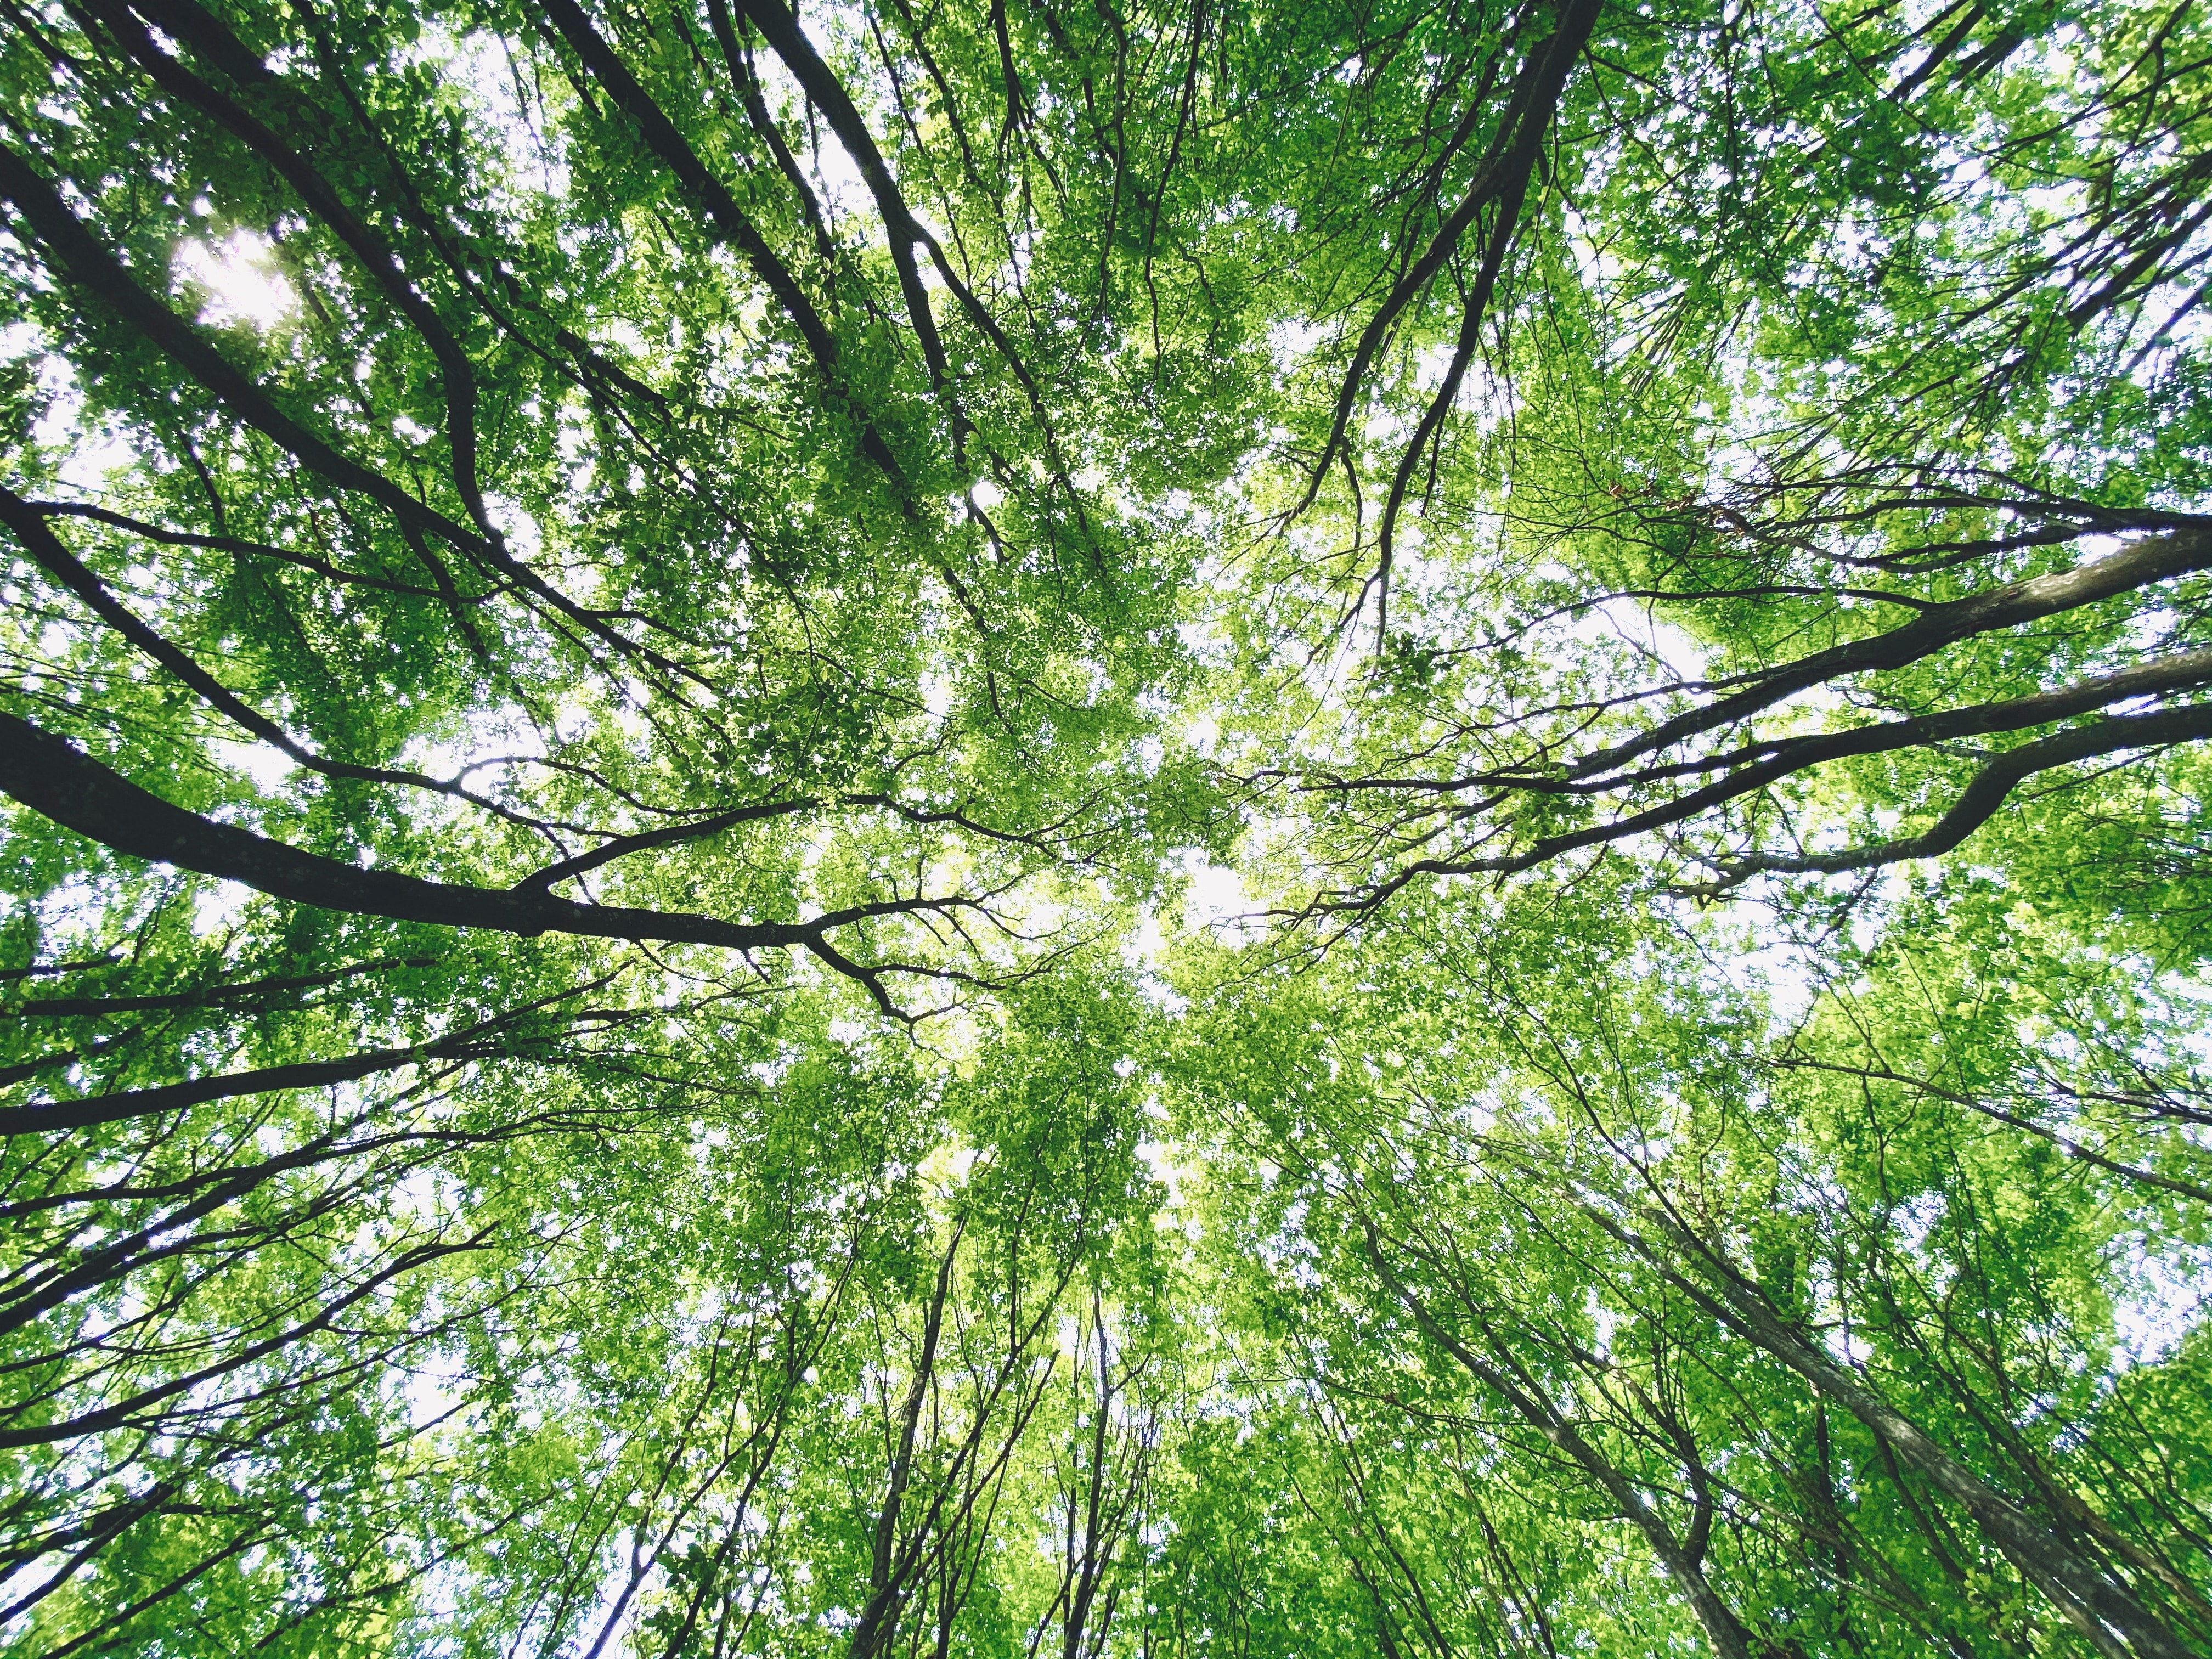
\includegraphics[width=12cm]{assets/misc/example.jpg}}
\author{
    Lily Leewis\\
    $$\href{mailto:lily.leewis@student.hu.nl}{lily.leewis@student.hu.nl}$$\\
    1st year open-ict student\\
    \newline
}

\fancyhf{}
\renewcommand{\headrulewidth}{2pt}
\renewcommand{\footrulewidth}{1pt}
\lhead{L. Leewis(1858379)}
\rhead{
    
\includegraphics[width = 3cm]{assets/HU/logo.png}
    }
\lfoot{Pagina \thepage\space van \pageref{LastPage}}
